% Minimal Beamer example for mediatr TikZ diagrams
% For slides/presentations
\documentclass[12pt]{beamer}

% === Required for mediatr diagrams ===
\usepackage{tikz}
\usetikzlibrary{arrows.meta}
\usepackage{xcolor}

\usetheme{default}
\setbeamertemplate{navigation symbols}{}

\title{Mediation Analysis}
\author{Your Name}
\date{\today}

\begin{document}

\begin{frame}[shrink=20]
\frametitle{Mediation Results}

% Option 1: Input from external file
% \input{my_diagram.tex}

% Option 2: Inline (what med_diagram_acme_tikz generates with mode="slide")
\begin{figure}
\begin{center}
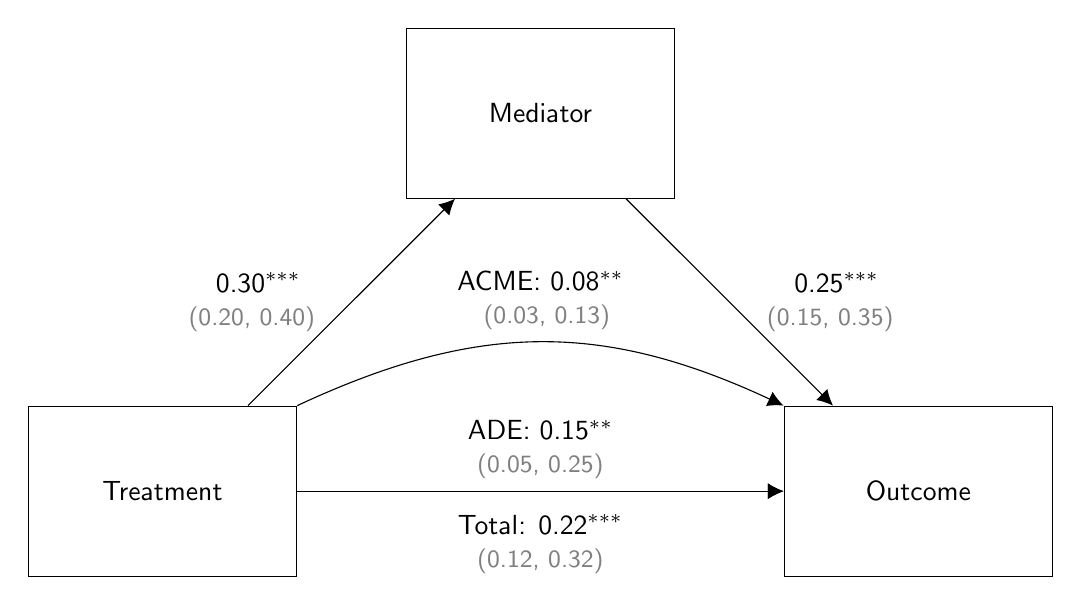
\begin{tikzpicture}[scale=0.8, >=stealth, font=\sffamily]
\normalsize
\tikzset{mynode/.style={draw, text centered, text width = 1.25in, minimum height = .85in, align=center} }
\tikzset{>={Latex[width=2mm,length=2mm]}}
\node[mynode] (x) at (0,0)  {Treatment};
\node[mynode] (y) at (12,0) {Outcome};
\node[mynode] (m) at (6,6)  {Mediator};
\path[->] (x) edge node[above, align=center, yshift=1pt] {ADE: 0.15$^{**}$ \\ \textcolor{gray}{\small{(0.05, 0.25)}} } (y);
\path[->] (x) edge node[left, align=center, xshift=-5pt] {0.30$^{***}$ \\ \textcolor{gray}{\small{(0.20, 0.40)\,\,\,}}} (m);
\path[->] (m) edge node[right, align=center, xshift=10pt] {0.25$^{***}$ \\ \textcolor{gray}{\small{(0.15, 0.35)\,\,\,}}} (y);
\path[->] (x) edge node[below, align=center, yshift=-5pt] {Total: 0.22$^{***}$ \\ \textcolor{gray}{\small{(0.12, 0.32)}}} (y);
\draw[->] (x.north east) to[out=25, in=155, looseness=1.05] node[midway, above, align=center, yshift=1pt] {ACME: 0.08$^{**}$ \\ \textcolor{gray}{\small{\,\,\,(0.03, 0.13)}}} (y.north west);
\end{tikzpicture}
\end{center}
\end{figure}

\end{frame}

\end{document}
